\documentclass[10pt,journal,compsoc]{IEEEtran}

\usepackage{amsmath,amssymb,amsthm}
\usepackage{graphicx}
\usepackage{booktabs}
\usepackage{hyperref}
\usepackage{enumitem}
\usepackage{algorithm}
\usepackage{algorithmic}
\usepackage{tikz}
\usetikzlibrary{arrows.meta,positioning,shapes}

\newtheorem{theorem}{Theorem}
\newtheorem{definition}{Definition}
\newtheorem{corollary}{Corollary}
\newtheorem{remark}{Remark}

\hypersetup{colorlinks=true,linkcolor=blue,citecolor=blue,urlcolor=blue}

\begin{document}

\title{Crash-Consistent Checkpointing for Exactly-Once Agent Effects:\\
A Write-Ahead Claim Log for LLM Agent Harnesses}

\author{Mohammed~Kamran~Syed%
\thanks{Manuscript draft, October 2026.}%
}

\markboth{IEEE Transactions on Parallel and Distributed Systems}%
{M.\ K.\ Syed: Crash-Consistent Checkpointing for Exactly-Once Agent Effects}

\maketitle

\begin{abstract}
LLM agent harnesses checkpoint \emph{trajectories}, not \emph{effect
commitments}. When the harness process crashes in the window between a
tool-effect commit and the checkpoint write, the resumed agent re-fires
the tool, producing a duplicate side effect---the ``double refund''
window. We show that idempotency keys alone cannot close this window in
general: content-hash keys break when the recovered agent rewords
arguments on retry, and deterministic $(\mathit{workflow},\mathit{step},
\mathit{action})$ keys break when recovery replanning shifts step
indices. We prove this insufficiency formally and propose a
\emph{write-ahead effect-claim log}: the claim and its key are logged
durably \emph{before} the tool is invoked, checkpoints are fenced by the
log, and recovery reconciles from the log first, guarded by a fencing
epoch against stale writers. Across a scripted sandbox (1,500
episodes/condition), two-model LLM validation (140 episodes: 70 per model; 210 including the tight-prompt ablation),
component ablations, and a production-shaped LangGraph deployment with
real \texttt{SIGKILL} fault injection---including a real-LLM supervisor
under uniform and mixed routing distributions---the protocol commits
\emph{zero duplicate effects} in every campaign (one-sided exact 95\%
upper bounds: 4.87\% at $n{=}60$, 0.20\% at $n{=}1{,}500$), where the
baseline duplicates at 0.77--0.83 and idempotency keys at 0.21--0.37.
Workflow completion (every accepted effect committed exactly once)
reaches 1.000 in the sandbox, the LangGraph campaigns, and LLM
validation with gpt-4.1-mini (70/70) and with a tightened recovery
prompt for gpt-4o-mini (70/70); under the loose prompt gpt-4o-mini
completes 66/70, the 4 misses being prompt-fixable model
re-emission loops, never duplicate commits. Claim-log write latency
is p50 20.3\,ms per step (fsync'd Claim/Commit records).
\end{abstract}

\begin{IEEEkeywords}
Fault tolerance, crash consistency, exactly-once semantics,
write-ahead logging, LLM agents, checkpoint-restart, idempotency,
fencing.
\end{IEEEkeywords}

\section{Introduction}
\label{sec:intro}

A customer support agent issues a \$212 refund, then its harness
process is OOM-killed. The harness restarts, loads its last
checkpoint---which was written \emph{before} the refund tool
returned---and, seeing no record of the refund, issues it again.
The customer is refunded twice. The ledger shows two commits; the
checkpoint shows one intent. Nobody is at fault except the
architecture: the harness checkpointed the agent's \emph{trajectory}
(messages, tool-call records) but not the world's \emph{commitments}.

This is the normal operating picture for modern agent harnesses.
LangGraph, CrewAI, AutoGen, and the OpenAI Agents SDK all persist
enough state to resume a conversation after a crash. None of them,
as of this writing, provides crash-consistent exactly-once
semantics for \emph{external side effects}. Production documentation
acknowledges the gap plainly: work performed between the last
checkpoint and a crash ``can run again'' for external effects.
Independent measurements confirm that LangGraph re-executes
durably recorded work after real process kills~\cite{khan2026resume}.
As agents move from demos to production---handling money,
sending customer-facing email, mutating systems of record---the
``double refund'' window stops being an edge case and becomes a
correctness bug with financial and legal consequences.

The database community solved the analogous problem decades ago
with write-ahead logging (WAL): never mutate state without first
durably recording the intent, so recovery can reconcile. But the
agent setting breaks a load-bearing assumption of classical WAL.
In a database, the writer never re-synthesizes its own transaction
identity after a crash; the log record and the retry trivially
coincide. In an agent harness, the \emph{recovered agent is an LLM}
that re-plans: it rewords arguments, inserts diagnostic steps,
reorders its plan. Any recovery scheme that depends on the
recovered agent re-deriving the \emph{same} effect identity it
used before the crash is fragile by construction---and, as we
prove in \S\ref{sec:formal}, fragile \emph{in general}, not just
in practice.

The industry-standard remedy is idempotency keys: attach a key to
each tool call so the tool can suppress repeats. Keys help---we
measure duplicate rates falling from 0.77 to 0.21--0.37---but they
fail exactly where LLM re-synthesis is most characteristic. A
content-hash key over the arguments breaks when the recovered
agent rewords them (observed reword rate 50\% in our scripted
recovery, 11\% with real models). A deterministic key derived
from $(\mathit{workflow\_id}, \mathit{step\_index},
\mathit{action})$ breaks when recovery replanning shifts step
indices (observed 30\% plan-shift rate). In both cases the retry
presents a key the tool has never seen, the tool commits again,
and the duplicate lands. The failure is structural: keys-alone
pushes all of recovery correctness into a value re-derived
\emph{after} the crash, by an agent whose re-synthesis the
harness cannot constrain.

This paper makes three contributions.

\textbf{(1) A fault class.} We formalize the \emph{checkpoint
window} $W(s) = (t_{\mathrm{commit}}(s), t_{\mathrm{ckpt}}(s))$:
the open interval between a tool-effect commit and the harness
checkpoint write for step~$s$. This is a \emph{harness-side}
crash-consistency gap, distinct from the service-boundary
late-commit window studied in recent agent fault-injection
work~\cite{limbo2026}: there the uncertainty is \emph{whether the
service committed}; here the tool \emph{has} committed and the
uncertainty is \emph{whether the harness recorded it}. The
distinction determines the fix.

\textbf{(2) A mechanism with a necessity proof.} We propose the
\emph{write-ahead effect-claim log}: before invoking a tool, the
harness durably logs a \textsc{Claim} carrying the effect's
identity and key; checkpoints may advance only past logged
\textsc{Commit} records (\emph{log-fenced checkpoints}); recovery
reconciles from the log \emph{first}, replaying uncommitted claims
with their original keys, under a fencing epoch that rejects stale
pre-crash writers. We prove (Theorem~1) that idempotency-key derivations computed
at retry time from \emph{mutable} inputs---rewordable argument
text, shiftable plan positions---cannot guarantee duplicate
suppression across all admissible recovery replans, and show
empirically where that boundary lies (E2a/E2b); durable
write-ahead identity information is the necessary ingredient,
and our claim log is a sufficient mechanism. Theorem~2 then
separates what the protocol guarantees: at-most-once commitment
per durable claim identity (safety), eventual commitment of
accepted claims under explicit progress assumptions, and
workflow completion as a property of the planning policy, not
the protocol.

\textbf{(3) Measurement.} We evaluate across four layers: a
scripted sandbox (1,500 episodes per condition) isolating the
fault; two-model LLM-driven validation (140 episodes: 70 per model), plus a
70-episode tight-prompt ablation (210 LLM episodes total) with real
model re-synthesis on recovery; component ablations proving each
protocol piece load-bearing against disjoint failure modes; and a
production-shaped LangGraph deployment (branching supervisor,
parallel fan-out, retries) with real \texttt{SIGKILL} fault
injection, including a real-LLM supervisor variant under both
uniform and mixed routing distributions. The write-ahead log
achieves \textbf{0.000} duplicate-effect rate and \textbf{1.000}
exactly-once rate in every campaign, against baseline duplicate
rates of 0.77--0.83 and idempotency-key rates of 0.21--0.37.
Claim-log overhead is p50 20.3\,ms per step---about a 1\% tax on
multi-second agentic steps.

The remainder of this paper is organized as follows.
\S\ref{sec:related} surveys related work and positions this paper
against the nearest neighbors. \S\ref{sec:problem} formalizes the
checkpoint window and walks through a concrete failure.
\S\ref{sec:design} presents the protocol, its record format, and
the reconciliation algorithm. \S\ref{sec:formal} gives the fault
model, both theorems, and honest limits. \S\ref{sec:eval} and
\S\ref{sec:ablation} report the evaluation and ablations;
\S\ref{sec:discussion} discusses the key-derivation boundary our
results reveal; \S\ref{sec:limitations} states the limitations;
\S\ref{sec:conclusion} concludes.

\section{Background and Related Work}
\label{sec:related}

\subsection{Idempotency keys for agent tools}

The closest empirical work is Li's \emph{Where Does Exactly-Once Live?}~\cite{limbo2026}
(whose sandbox is named Limbo), which
applies idempotency keys to agent tool calls and measures
duplicate reduction from 28\% to 4\% across 12 injected fault
modes. Its contribution is real, but its fault taxonomy is
service-boundary throughout: the late-commit window it studies is
the interval between the agent's dispatch and the service's commit
becoming visible---the uncertainty is \emph{whether the service
committed}. Its full text contains zero mentions of ``crash'' or
``write-ahead''; the harness-side checkpoint window is untested
there. Our work is complementary: Li measures what keys achieve
at the service boundary; we show where keys fail at the harness
boundary and what structure is needed instead. We adopt the same
tool-contract idealization (atomic check-and-commit) as shared
ground. Its residual 4\% lives at the \emph{service} boundary
(late commits, in-flight ambiguity across its twelve fault
modes), a different fault class from our harness-side
commit$\to$checkpoint window; we do not claim to explain it.
What transfers is the lesson: wherever recovery correctness
depends on re-deriving an identity after the failure, some
residual remains, and only durable records close it.

\subsection{Crash and rollback in agent frameworks}

Three recent papers are adjacent must-cites. Khan's \emph{Resume
Means Resume}~\cite{khan2026resume} gives a machine-checked
(TLA+/TLAPS) resume contract for workflow persistence layers and
independently measures LangGraph re-executing durably recorded
work after real \texttt{SIGKILL}---direct confirmation of the
baseline fault our sandbox reproduces (0.80 duplicate rate). Where
Khan specifies what resume \emph{must mean}, we show \emph{how to
achieve} exactly-once for the commit$\to$checkpoint window and
measure it: contract and mechanism, complementary. Zheng et
al.~\cite{zheng2026checkpoint} formalize exact checking of
execution edits (checkpoint/fork/restore/merge) in Lean, noting
that unsafe edits can ``authorize the same tool action twice'';
their solution is a decision procedure for edit safety, not a
crash-consistency mechanism. \emph{Safe to Resume?}
~\cite{safutoresume2026} documents five rollback failure modes
including unrecorded external effects with a duplicate-payment
demonstration on LangGraph, under an adversarial framing.
ACRFence~\cite{acrfence2026} is the closest adjacent mechanism:
it \emph{records irreversible tool effects} and enforces
replay-or-fork semantics upon restore, which overlaps with our
durable effect records in purpose if not in form. The
differences are the threat model---semantic rollback
\emph{attacks} (Action Replay, Authority Resurrection) versus
our benign crash-stop fault---and the mechanism: ACRFence
constrains what a \emph{restored} agent may re-issue, while our
write-ahead claim log plus reconciliation-first recovery and
epoch fencing make re-issuance unnecessary in the first place.
Our fault model is deliberately benign (crash-stop, chaos/HPC
checkpoint-restart tradition); there is no adversary in this
paper. AgentRewind~\cite{agentrewind2026} records aligned
checkpoints of agent context and controlled environment for
long-horizon recovery, but explicitly cannot undo external
effects: the opposite direction from ours.

\subsection{Logs for agents}

LogAct~\cite{logact2026} is the closest published neighbor in
spirit: it structures agents as state machines playing a shared,
append-only AgentBus and explicitly discusses crash recovery via
the bus as a write-ahead log, including fencing of stale (old-driver)
writers after a crash. Its focus, however, is a \emph{shared}
multi-agent bus with pre-execution voting, semantic (LLM-driven)
recovery, and introspection---not the single-harness
commit$\to$checkpoint window or exactly-once effect semantics
under crash, which it does not measure. Our claim log is a
per-harness write-ahead \emph{effect-claim} log paired with
log-fenced checkpoints and reconciliation-first recovery; where
LogAct's bus mediates among deconstructed agent roles, our log
mediates between one crash-prone harness and its tools. A
formal-methods treatment of the checkpoint crash window exists in
the distributed-systems literature as an impossibility-style
result, but without agents, LLMs, tools that keep their own
records, or a mechanism; we cite it as the closest formal
neighbor and distinguish our constructive, measured
contribution.

\subsection{Durable execution and sagas}

The systems lineage is write-ahead logging and durable
execution. The canonical WAL treatment is ARIES~\cite{aries1992}:
never mutate state without first durably recording the intent,
so recovery can reconcile---the discipline our claim log adapts.
Classical WAL assumes a writer that never re-synthesizes its own
operation identity after a crash; the log record and the retry
trivially coincide. RIFL~\cite{rifl2015} is the closest
classical analogue to our receiver contract: it converts
at-least-once RPCs to exactly-once by durably recording
completed-call results and returning the original result on
retry, migrating that metadata with the data across
reconfiguration. Our tool-side idempotent receiver (\S\ref{sec:design}) follows
the same idea at the harness/tool boundary, though our current
contract returns status only on duplicates---original-result return
is specified future work (\S\ref{sec:limitations}); what is new is
the \emph{harness-side} half of the problem---the recovered
agent is an LLM that re-plans, rewords, and re-indexes, so the
retry may never present the recorded identity at all. No
receiver-side mechanism alone (RIFL included) can suppress a
retry it cannot recognize; the claim log's
\textsc{find\_by\_identity} reconciliation exists precisely to
re-attach the original identity before the tool is consulted.
Modern durable execution (Temporal, DBOS-style) gives
exactly-once workflow execution via durable logs and replay but
likewise assumes deterministic re-derivation on replay---no
post-crash identity re-synthesis. Our adaptation---semantic
claim identity, log-fenced checkpoints, and epoch fencing at
the harness/tool boundary, under LLM re-synthesis
nondeterminism---is the non-trivial part, and the measured gap
it closes (0.000 vs.\ 0.21--0.77) is the contribution. The saga
pattern~\cite{sagas1987} addresses multi-step transaction
compensation (semantic atomicity across services), a different
correctness property from exactly-once of individual effects;
our protocol composes with saga-style compensation (the claim
log is a natural saga journal) but does not require it.

In sum: no prior work combines the benign commit$\to$checkpoint
crash window as the fault, a write-ahead effect-claim log with
reconciliation-first recovery as the fix, measured zero
duplicates at exactly-once 1.000, and an analysis of
idempotency-key fragility under rewording and plan shift. A
pre-submission literature re-check (October 2026) confirmed this
against the active 2026 literature, which clusters around
adversarial rollback, formal contracts and checking, sandbox
checkpoint/restore, and oversight logging---all adjacent problems
or different solutions.

\begin{table*}[t]
\centering
\caption{Positioning: fault model, durable records, identity handling,
receiver assumptions, fencing, guarantee, and evaluation across adjacent work.
``Harness-side'' = the commit$\to$checkpoint window $W(s)$; ``service-side'' =
the dispatch$\to$commit visibility window.}
\label{tab:positioning}
\begin{tabular}{p{1.9cm}p{1.9cm}p{2.0cm}p{2.0cm}p{2.0cm}p{1.7cm}p{1.9cm}p{2.0cm}}
\toprule
Work & Fault model & Durable records & Identity handling & Receiver assumptions & Fencing & Guarantee & Evaluation \\
\midrule
This paper &
Benign crash-stop, harness-side $W(s)$ &
Per-harness write-ahead effect-claim log; log-fenced checkpoints &
Semantic $(\mathit{action},\mathit{target})$ reconciliation; original keys replayed, never re-derived &
Idempotent, atomic check-and-commit; returns original result on duplicate &
Epoch fencing vs.\ stale pre-crash writers &
Exactly-once per durable claim identity (safety); 0 duplicates measured &
1,500 eps/cond sandbox; 210 LLM eps; 60 eps/cond LangGraph + real SIGKILL; ablations; E1--E4 boundary experiments \\
\midrule
Li~\cite{limbo2026} (``Limbo'' sandbox) &
Service-side: timeouts, late commits, redelivery; benign &
Ledger of committed effects (grading oracle), per-service idempotency-key sets &
Keys attached by harness guard; agent re-synthesis out of scope &
Optional idempotency keys; eventually consistent / missing read paths &
None &
Measured: keys cut duplicates 28\%$\to$4\%; no exact-once proof &
25,930 eps; 9 models; 3 harnesses; 12 fault modes; 15 recovery conditions \\
\midrule
ACRFence~\cite{acrfence2026} &
\emph{Adversarial} rollback (Action Replay, Authority Resurrection) &
Record of irreversible tool effects &
Re-synthesized requests treated as new by servers (the attack) &
Server-side replay-or-fork enforcement &
Implicit in replay-or-fork &
Mitigation of semantic rollback attacks &
PoC experiments \\
\midrule
LogAct~\cite{logact2026} &
Crash-stop (agent or environment), benign &
Shared append-only AgentBus (WAL discipline); old-driver fencing &
State-machine replay from bus; semantic (LLM) recovery &
Voters approve pre-execution; executors typed &
Old-driver fencing on the bus &
Consistent recovery; attack blocking (3\% benign-utility cost) &
Benchmarks: recovery correctness, token savings, attack blocking \\
\midrule
AgentRewind~\cite{agentrewind2026} &
Errors propagating through context/environment &
Aligned checkpoints of agent context + controlled environment &
Resume with prior-attempt information &
Controlled environment only &
None &
Improved task success / checklist progress &
MettleBench long-horizon tasks \\
\midrule
Safe to Resume?~\cite{safutoresume2026} &
\emph{Adversarial} rollback; 5 failure modes incl.\ unrecorded external effects &
Varies by framework (the gap under study) &
Nondeterministic replay characterized &
Framework-dependent &
None (failure mode) &
None---documents failures; double-payment demo &
5 frameworks; 3 end-to-end attacks \\
\midrule
Khan~\cite{khan2026resume} &
Crash-stop resume &
Workflow persistence layer &
N/A (contract level) &
N/A &
N/A &
Machine-checked (TLA+/TLAPS) resume contract &
LangGraph re-execution measurement \\
\midrule
RIFL~\cite{rifl2015} &
Server crash, benign &
Durable completed-RPC result records, migrated with data &
Client-supplied request IDs; retry recognized by ID &
Returns saved result on duplicate; lease-GC'd metadata &
N/A (no stale writers) &
Linearizability (exactly-once RPC) &
RAMCloud: $<$4\% overhead \\
\midrule
ARIES~\cite{aries1992} &
System crash, benign &
WAL; dirty-page table; checkpoints &
LSN-identified log records; no re-synthesis &
Page-level redo/undo &
N/A &
Atomicity + durability (analysis/redo/undo) &
Analytical; systems at IBM \\
\midrule
Sagas~\cite{sagas1987} &
Step failure, benign &
Saga log; compensating transactions &
Saga/step IDs; no re-synthesis &
Compensating actions defined per step &
N/A &
Semantic atomicity (all-or-compensated) &
Analytical \\
\bottomrule
\end{tabular}
\end{table*}

\section{The Checkpoint Window}
\label{sec:problem}

\subsection{A concrete failure}

Consider a three-step customer-support workflow: (1) look up the
order (read-only), (2) issue a \$212 refund via
\texttt{payments.refund} (non-idempotent), (3) send a
confirmation email. The harness executes step~2: the tool commits
(the money moves), and the harness prepares to write its
checkpoint. Between those two events, the container is
OOM-killed. On restart, the harness loads its last durable
checkpoint, which records the workflow as ``step~2 pending.''
The agent---a fresh LLM generation with no memory of the
kill---reasons that the refund was never issued and fires
\texttt{payments.refund} again. The tool, seeing a new request
(or a re-derived key it does not recognize), commits again.
Two refunds; one checkpoint.

Note what did \emph{not} fail: the tool behaved correctly, the
checkpoint logic behaved correctly, and the agent behaved
rationally given its state. The fault is architectural: the
durable state records \emph{intent} while the world records
\emph{commitment}, and nothing durable bridges them.

\subsection{Formalization}

Consider an agent harness $H$ executing a workflow of effectful
steps against external tools $T$ (durably recording every
committed effect). For step $s$, order the relevant events:
$t_{\mathrm{claim}}(s) < t_{\mathrm{call}}(s) \le
t_{\mathrm{commit}}(s) < t_{\mathrm{mark}}(s) <
t_{\mathrm{ckpt}}(s)$: the effect is claimed, the tool invoked,
the effect committed (the real world changes), the commit
recorded, the checkpoint advanced.

\begin{definition}[Checkpoint window]
$W(s) = (t_{\mathrm{commit}}(s), t_{\mathrm{ckpt}}(s))$: the open
interval between the tool-effect commit and the harness
checkpoint write for step $s$.
\end{definition}

A crash-stop failure of $H$ at time $t_c$ lands, for the step in
flight, in one of three places: \emph{pre-step}
($t_c < t_{\mathrm{commit}}(s)$, safe---the effect never
committed); \emph{in-window} ($t_c \in W(s)$, the fault under
study---the effect committed but the harness does not know it);
or \emph{post-checkpoint} ($t_c \ge t_{\mathrm{ckpt}}(s)$,
safe---commit recorded and checkpointed). Figure~\ref{fig:window}
shows the event timeline. Recovery from the last durable
checkpoint replays from before $s$; the agent re-fires the tool;
the effect duplicates.

\begin{figure}[ht]
\centering
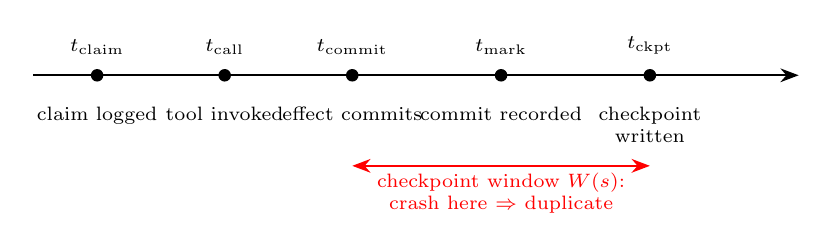
\begin{tikzpicture}[x=1.35cm,>=Stealth,
    event/.style={circle,fill=black,inner sep=1.6pt},
    lbl/.style={font=\scriptsize,align=center}]
\draw[->,thick] (0,0) -- (7.2,0);
\foreach \x/\t/\l in {0.6/$t_{\mathrm{claim}}$/claim logged,
    1.8/$t_{\mathrm{call}}$/tool invoked,
    3.0/$t_{\mathrm{commit}}$/effect commits,
    4.4/$t_{\mathrm{mark}}$/commit recorded,
    5.8/$t_{\mathrm{ckpt}}$/checkpoint\\written} {
  \node[event] at (\x,0) {};
  \node[lbl,above=4pt] at (\x,0) {\t};
  \node[lbl,below=8pt] at (\x,0) {\l};
}
\draw[<->,thick,red] (3.0,-1.15) -- (5.8,-1.15);
\node[lbl,red] at (4.4,-1.5) {checkpoint window $W(s)$:\\crash here $\Rightarrow$ duplicate};
\end{tikzpicture}
\caption{Event timeline for an effectful step. A crash landing
in $W(s)$---after the real-world commit but before the
checkpoint write---is the fault under study.}
\label{fig:window}
\end{figure}

Two properties make this window specifically an \emph{agent}
problem rather than a classical database problem. First, the
recovered agent re-synthesizes its plan with an LLM: arguments
get reworded, steps get inserted or reordered. Any recovery
scheme that depends on the recovered agent re-deriving the
\emph{same} effect identity is fragile by construction. Second,
classical write-ahead logging assumes the writer never
re-synthesizes its own transaction identity after a crash; the
agent harness violates that assumption routinely. The fix must
therefore make recovery \emph{independent} of the agent's
post-crash re-derivation.

\section{Design: The Write-Ahead Effect-Claim Protocol}
\label{sec:design}

\subsection{Principals and record format}

\emph{Principals.} $H$: the crash-prone agent harness process.
$T$: the external tool/service, durable across $H$ crashes, and
an \emph{atomic idempotent receiver}: $T.\mathrm{call}(k, e,
\mathit{args})$ atomically checks whether key $k$ was seen and
commits the effect iff not, returning \textsc{committed} or
\textsc{duplicate\_suppressed} (status only; the original result
payload is not returned — §\ref{sec:limitations}). It keeps a durable
per-workflow key set and a per-workflow fencing epoch
$\mathit{max\_epoch}$, rejecting calls with $e <
\mathit{max\_epoch}$. Fence acquisition is
$\mathit{max}$-monotonic at $T$: the durable arbiter of the
current epoch is $T$, not the harness's local epoch file. $L$: the
write-ahead effect-claim log, durable (fsync'd append-only JSONL
in our implementation, $\sim$376 bytes per step). $C$: the
checkpoint (last fully-recorded step index), durable.

Each claim record carries the fields in Table~\ref{tab:record}:
the workflow and step identity, the key fixed at claim time, the
arguments as invoked, the fencing epoch, and the record type.
The key need only be deterministic \emph{at claim time}---post-crash
re-derivability is irrelevant, because the log supplies the key
(see Remark~1).

\begin{table}[ht]
\centering
\caption{Claim-log record format.}
\label{tab:record}
\begin{tabular}{ll}
\toprule
Field & Purpose \\
\midrule
\texttt{wid} & Workflow identifier \\
\texttt{step} & Step index within the workflow \\
\texttt{key} & Idempotency key, fixed at claim time \\
\texttt{action}, \texttt{target} & Semantic claim identity \\
\texttt{args} & Arguments as invoked \\
\texttt{epoch} & Fencing epoch of the claiming generation \\
\texttt{type} & \textsc{Claim} or \textsc{Commit} \\
\bottomrule
\end{tabular}
\end{table}

\emph{Claim discipline.} $H$ never invokes $T$ without a prior
durable $\textsc{Claim}(\mathit{wid}, s, k(s), \mathit{args},
\mathit{epoch})$ in $L$. This is harness-\emph{enforced}: the
harness refuses the tool call otherwise. In our LLM validation
the discipline held at 98.3\% of steps (100\% of episodes);
violations degrade to \emph{refused calls}---the safe direction
(missing, never duplicates).

\subsection{Normal and recovery paths}

\emph{Normal path} for an effectful step $s$:
\begin{enumerate}[nosep]
\item $H$ appends $\textsc{Claim}(s)$ to $L$ (\emph{write-ahead}).
\item $H$ invokes $T.\mathrm{call}(k(s), \mathit{epoch},
\mathit{args})$.
\item $H$ appends $\textsc{Commit}(s)$ to $L$, then advances $C$
past $s$. $C$ may advance past $s$ \textbf{only if}
$\textsc{Commit}(s) \in L$ (\emph{log-fenced checkpoint}).
\end{enumerate}

\emph{Recovery path} ($H$ restarts; only $L$, $C$, $T$ survive)
is given as Algorithm~\ref{alg:recover}.

\begin{algorithm}[t]
\caption{Reconciliation-first recovery}
\label{alg:recover}
\begin{algorithmic}[1]
\STATE $\mathit{epoch} \gets \mathrm{CAS}_{T}(\mathit{epoch}+1)$
\COMMENT{atomic fence acquisition at $T$; single-recovery-writer
assumed in our implementation (\S\ref{sec:design})}
\FOR{each $\textsc{Claim}(s) \in L$ without matching
\textsc{Commit}}
\STATE $T.\mathrm{call}(k(s), \mathit{epoch},
\mathit{args}(s))$ \COMMENT{original key from $L$}
\STATE append $\textsc{Commit}(s)$ on success
\ENDFOR
\STATE advance $C$ past all \textsc{Commit}ted claims
\COMMENT{log-fenced}
\STATE resume agent from $C$; check post-recovery steps
against $L$ by $(\mathit{action}, \mathit{target})$ before
issuing new claims \COMMENT{semantic skip}
\end{algorithmic}
\end{algorithm}

A torn trailing record in $L$ is skipped on load (standard WAL tail
discipline); a torn non-trailing record is treated as corruption. A torn
\textsc{Commit} is safe: the claim replays with its original key and $T$
suppresses it.

Three design points deserve emphasis. Figure~\ref{fig:arch}
summarizes the architecture. First, reconciliation uses
the claim's \emph{original} key from $L$---the agent is never
required to re-derive a key, which is precisely where keys-alone
fails (\S\ref{sec:formal}). The tool's idempotent receiver
dedups if the pre-crash call committed, executes if it never
arrived: exactly-once either way. Second, the fencing epoch
closes the \emph{zombie writer} hole: a pre-crash in-flight call
arriving after recovery bears a stale epoch and is rejected, so
no phantom commit can slip in after reconciliation. This holds under the
crash-stop fault model with a single recovery writer per crash: epoch
acquisition is read-increment-write on the harness side and atomic only
via $T$'s $\mathit{max}$-monotonic fence; two concurrent recoveries could
share an epoch (see \S\ref{sec:limitations}). Third,
log-fenced checkpoints preserve the protocol's core
invariant---$C$ never runs ahead of $L$---so the checkpoint
window $W(s)$ is the \emph{only} place an in-window crash can
land, and reconciliation covers exactly that window.

The semantic skip in line~7 of Algorithm~\ref{alg:recover}
handles the LLM re-synthesis problem: post-recovery steps are
checked against $L$ by $(\mathit{action}, \mathit{target})$
before any new claim issues, so reworded or re-indexed retries
of already-claimed effects are skipped rather than re-executed.

\emph{Parallel execution.} Fan-out uses one durable file per settled branch
rather than a single checkpoint record, so concurrent workers never race on
a read-modify-write checkpoint; the completion frontier is the \emph{set} of
settled branches and tolerates gaps. Recovery recomputes the frontier from
$L$ under the log-fenced rule: a branch is settled only if \emph{every} one
of its effects has a matching \textsc{Commit}. The protocol currently
assumes disjoint effect ownership across parallel workers: two workers
concurrently claiming the same $(\mathit{action}, \mathit{target})$ are not
serialized by the log, and the receiver dedups by key, not by identity
(see \S\ref{sec:limitations}).

\begin{figure}[ht]
\centering
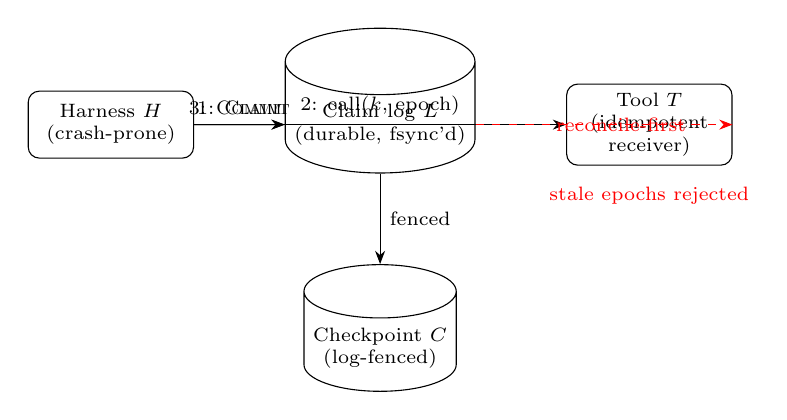
\begin{tikzpicture}[>=Stealth,node distance=1.15cm,
    box/.style={rectangle,draw,rounded corners,align=center,
      font=\scriptsize,minimum width=2.1cm,minimum height=0.85cm},
    db/.style={cylinder,draw,shape border rotate=90,align=center,
      font=\scriptsize,minimum width=1.7cm,minimum height=1.0cm,
      aspect=0.35}]
\node[box] (h) {Harness $H$\\(crash-prone)};
\node[db,right=of h] (l) {Claim log $L$\\(durable, fsync'd)};
\node[db,below=of l] (c) {Checkpoint $C$\\(log-fenced)};
\node[box,right=of l] (t) {Tool $T$\\(idempotent\\receiver)};
\draw[->] (h) -- node[font=\scriptsize,above] {1: \textsc{Claim}} (l);
\draw[->] (h.east) -- node[font=\scriptsize,above] {2: call($k$, epoch)} (t.west);
\draw[->] (h) -- node[font=\scriptsize,above] {3: \textsc{Commit}} (l);
\draw[->] (l) -- node[font=\scriptsize,right] {fenced} (c);
\draw[->,dashed,red] (l.east) -- ++(0.9,0) |- node[font=\scriptsize,
  near start,right] {reconcile-first} (t.east);
\node[font=\scriptsize,red,below=0.15cm of t] {stale epochs rejected};
\end{tikzpicture}
\caption{Protocol architecture. The harness claims before
invoking (1--2), commits after (3); checkpoints advance only
past logged commits. Recovery reconciles from the log first
(dashed), replaying original keys under a fresh fencing epoch.}
\label{fig:arch}
\end{figure}

\subsection{Implementation notes}

Our reference implementation uses an fsync'd append-only JSONL
claim log ($\sim$376 bytes/step) and atomic checkpoint writes;
the tool side is a separate-process HTTP server implementing
atomic check-and-commit with per-workflow seen-key sets and
fencing epochs, plus an append-only ledger that serves as
ground truth for scoring. The LangGraph port
(\S\ref{sec:eval}) reuses the same record shape and
discipline inside a real \texttt{StateGraph}, with per-branch
claims for fan-out. Crash injection is a real
\texttt{SIGKILL} from an external watchdog process that
observes progress markers only---it shares no state with the
agent. Total API spend across all LLM campaigns was \$0.114
(\$0.095 for the three 70-episode validation runs, \$0.019 for
the two LangGraph supervisor campaigns).

\section{Formal Analysis}
\label{sec:formal}

\subsection{Fault model}

Crash-stop failure of $H$ only (benign faults, in the
chaos/HPC checkpoint-restart tradition); $L$, $C$, $T$ persist;
$T$ itself does not crash; no Byzantine behavior. One crash per
episode in our evaluation (the single-crash model standard in
checkpoint-restart studies).

\subsection{Necessity: keys alone cannot suffice}

\begin{theorem}[Retry-time key fragility]
Let $K$ be an idempotency-key derivation computed by the
\emph{recovered} agent at retry time from retry-time inputs that
are \emph{mutable under re-synthesis}---argument text the agent
may reword, or plan positions the recovery replan may shift. If
post-recovery re-synthesis is unconstrained over those
inputs, then a keys-only retry protocol cannot guarantee
duplicate suppression across all admissible recovery replans
under in-window crashes.
\end{theorem}

\begin{proof}[Proof sketch]
Fix a step $s$ committed in-window under $k = K(\text{pre-crash
inputs})$. Two admissible recoveries inside the mutable-input
class. (i) \emph{Content-hash keys}, $K = H(\mathit{action},
\mathit{args})$: the recovered agent rewords the arguments to
$a' \ne a$ (admissible). The retry presents
$k' = H(\mathit{action}, a') \ne k$; $T$ has never seen $k'$
and commits again---a duplicate. Empirical witness (E2b):
recovery-side rewording broke content-hash keys on 46/60
episodes (92 excess commits); the WAL held 60/60 via
canonicalized identity lookup. (ii) \emph{Deterministic
position keys}, $K = (\mathit{wid}, i, \mathit{action})$: the
recovered agent rotates branch indices on replan (admissible).
The retried logical step carries $i' \ne i$, so the retry
presents $k' = (\mathit{wid}, i', \mathit{action}) \ne k$---a
duplicate; symmetrically, a shifted retry whose new key
collides with an already-committed key is wrongly
suppressed---a lost effect. Empirical witness (E2a): positional
shift broke deterministic keys on 46/60 episodes with 46 missing
effects; the WAL held 60/60 via \texttt{find\_by\_identity} key
reuse. The failure is a property of the \emph{class}---retry-time
derivations from mutable inputs---not of the two schemes: any
$K$ in the class admits an admissible recovery with
$K' \ne K$, because the harness cannot constrain re-synthesis
inputs after the crash.
\end{proof}

\begin{remark}[Scope]
The theorem is silent on keys that are \emph{not} retry-time
derivations: durable business-operation IDs assigned by the tool
or domain and passed through unchanged lie outside its domain
and may suffice. This is exactly the boundary our evaluation
maps: under stable identities deterministic keys tie the WAL
(v2: 0.0000/1.0000 both; E1 native persistence 60/60); under
identity shift they fail (E2a/E2b).
\end{remark}

\begin{corollary}[Durable identity information]
The source of truth for effect identity must be fixed
\emph{before} the crash---a durable write-ahead identity record
binding the effect's logical identity to its key---not
re-derived after it. The \emph{information} (a durable
pre-commit identity record) is necessary; the append-only claim
log is a sufficient mechanism, not the unique one.
\end{corollary}

\emph{Empirical counterpart.} Scripted sandbox, 1,500
episodes/condition, in-window crash fraction 0.75:
duplicate-effect rates---baseline (no keys) 0.7687,
content-hash keys 0.3667, deterministic keys 0.2113,
write-ahead claim log \textbf{0.0000}. LangGraph production
port with real \texttt{SIGKILL}: under \emph{stable} identities
deterministic keys tie the WAL (0.0000/1.0000 both; E1 native
persistence likewise 60/60)---keys suffice there. Under
\emph{identity shift across recovery} (E2a positional, E2b
content rewording), deterministic keys break on 46/60 episodes
each while the WAL holds 60/60. The measured gap is the price
of re-derivation fragility, paid exactly where Theorem~1 says
it is due.

\begin{definition}[Logical effect identity]
A \emph{logical effect identity} is a function
$\mathit{id}: \mathcal{E} \to \mathcal{I}$ from tool effects to
an identity space, supplied per deployment, satisfying:
(i)~\emph{stability}---$\mathit{id}$ is invariant under argument
rewording and plan repositioning (business meaning, not surface
form); (ii)~\emph{discrimination}---distinct business intents
map to distinct identities even when $(\mathit{action},
\mathit{target})$ coincide (e.g., two separately authorized
refunds to the same recipient differ by an
occurrence/authorization component); (iii)~\emph{retry
equivalence}---a post-recovery retry $r$ of a claimed effect $c$
is \emph{equivalent} iff $\mathit{id}(r) = \mathit{id}(c)$;
equivalent retries must be suppressed, non-equivalent effects
must both commit. Default instantiation:
$\mathit{id} = (\mathit{action}, \mathit{target},
\mathit{occurrence})$. Misidentification breaks the protocol in
either direction; the identity function is a deployment
modeling assumption, not a theorem. All exactly-once claims
below are per \emph{durable claim identity} under the
deployment's $\mathit{id}$.
\end{definition}

\subsection{Correctness: the protocol guarantees exactly-once}

\begin{theorem}[At-most-once commitment]
Under (A1) atomic idempotent $T$, (A2) durable $L$ and $C$,
(A3) crash-stop $H$ only, (A4) epoch fencing, (A5) claim
discipline---for \textbf{any} crash time $t_c$ and
\textbf{any} post-recovery agent behavior, no durable claim
identity (per the deployment's $\mathit{id}$) commits more than
one tool effect.
\end{theorem}

\begin{theorem}[Eventual commitment of accepted claims]
Under (A1)--(A5) plus progress assumptions (P1) $T$ eventually
processes every call it accepts, (P2) the harness eventually
runs recovery to completion, (P3) fencing epochs are acquired
atomically---every \textsc{Claim} durably accepted into $L$ is
eventually committed by $T$. Accepted claims are at-least-once;
with Theorem~2a, exactly-once per claim identity.
\end{theorem}

\begin{remark}[Workflow completion is policy-dependent]
The protocol does \textbf{not} guarantee the agent emits the
remaining claims of a workflow; completion is a property of the
planning/recovery policy, not the protocol. The measured 66/70
completion (94.29\%, gpt-4o-mini; the 4 misses were model
re-emission loops, a supervisor-policy behavior) is an empirical
completion rate under a specific policy, not a liveness proof.
Safety held on all 70 episodes including the 4 incomplete ones:
0 duplicates.
\end{remark}

\begin{proof}[Proof sketch for at-most-once]
Case analysis on the crash landing for each step $s$, split at
every durability boundary. \emph{Case 1---before
\textsc{Claim} durable} ($t_c < t_{\mathrm{claim}}(s)$): no
durable trace exists; recovery treats $s$ as never attempted and
a fresh \textsc{Claim} with the claim-time key commits it once.
\emph{Case 2---\textsc{Claim} durable, call never arrived}
($t_c \in [t_{\mathrm{claim}}(s), t_{\mathrm{call}}(s))$):
reconciliation replays with the original key; $T$ has never seen
it and commits. \emph{Case 3---effect committed,
\textsc{Commit} not yet durable}
($t_c \in [t_{\mathrm{call}}(s), t_{\mathrm{mark}}(s))$): by
(A1) atomicity the effect committed exactly when the call
arrived, but $\textsc{Commit}(s) \notin L$. Reconciliation
replays with the original key; $T$ finds the key and suppresses
the duplicate; then \textsc{Commit} is written and $C$ advances
(log-fenced). This is the true in-window sub-case.
\emph{Case 4---\textsc{Commit} durable, checkpoint not yet
advanced} ($t_c \in [t_{\mathrm{mark}}(s),
t_{\mathrm{ckpt}}(s))$): $\textsc{Commit}(s) \in L$ but $C$ not
advanced past $s$. Reconciliation finds the
\textsc{Claim}+\textsc{Commit} pair and issues \emph{no replay};
$C$ advances past $s$. No duplicate, no loss. (The previous
version asserted $\textsc{Commit}(s) \notin L$ throughout $W(s)$;
since $t_{\mathrm{mark}} < t_{\mathrm{ckpt}}$, the sub-interval
$[t_{\mathrm{mark}}, t_{\mathrm{ckpt}}) \subset W(s)$ already has
the \textsc{Commit} durable. The old conclusion held---the
receiver suppresses by key either way---but the case analysis
was unsound as written; this split repairs it.)
\emph{Case 5---post-checkpoint} ($t_c \ge t_{\mathrm{ckpt}}(s)$):
$\textsc{Commit}(s) \in L$ and $C$ advanced; reconciliation
skips $s$ and the agent resumes after $C$. \emph{Stale writers:}
any in-flight pre-crash call arriving after recovery bears
$e < \mathit{max\_epoch}$ and is rejected by (A4); no zombie
commits (E4: 102/102 offending calls were this class; 0
same-key recommit attempts succeeded).
\emph{Agent-behavior independence:} reconciliation uses original
keys from $L$---the agent never re-derives a key---and
post-recovery steps are checked against $L$ by logical effect
identity before new claims issue, so reworded or shifted
retries of claimed effects are recognized as equivalent and
skipped. The argument holds for arbitrary post-recovery
behavior, including adversarial re-emission (observed: 11
consecutive re-emissions of committed effects, all suppressed,
0 duplicates over 70 LLM-driven episodes).
\end{proof}

\begin{proof}[Proof sketch for eventual commitment]
Reconciliation replays every \textsc{Claim} without a matching
\textsc{Commit} using its original key. By (P2) reconciliation
runs to completion; each replayed call either finds its key at
$T$ (already committed) or commits it (P1); (P3) guarantees the
replaying epoch owns the workflow. Hence every accepted claim
is eventually committed.
\end{proof}

\begin{remark}[Key determinism, sharpened]
The protocol requires keys to be deterministic only \emph{at
claim time} (so a pre-crash claim and any same-generation retry
coincide). Post-crash \emph{re-derivability} is irrelevant---the
log supplies the key. This is the precise point where keys-alone
fails and the write-ahead log succeeds.
\end{remark}

\subsection{Assumptions and limits}

\textbf{(L1) Tool idealization.} (A1) assumes atomic
check-and-commit at $T$. Real tools with non-atomic or
non-idempotent APIs need an adapter (e.g., a transactional
outbox at the tool boundary); the theorem does not cover them.
This is the same idealization as Li's tool contract---shared
ground, not a weakness unique to this work. \textbf{(L2) Log
durability.} (A2) is assumed, not proved; log loss voids the
guarantee---the standard WAL assumption, stated explicitly.
\textbf{(L3) Safety, not liveness.} Theorem~2 is a \emph{safety}
property (no duplicate commits; reconciliation gives
at-least-once of \emph{claimed} effects). It does not prove the
agent will emit remaining claims---completeness depends on agent
behavior and harness recovery policy. \textbf{(L4) Semantic
identity is a modeling choice.} Skip-logic keys on
$(\mathit{action}, \mathit{target})$ as the stable business
identity of an effect; effects whose identity cannot be captured
this way need a domain-specific identity function.
\textbf{(L5) Fault scope.} Crash-stop $H$ only; no Byzantine
harness, no tool-side crashes, single writer per workflow per
epoch (fencing enforces this). \textbf{(L6) Claim discipline is
enforced, not assumed.} (A5) held at 98.3\% step-level in LLM
validation because the harness \emph{refuses} tool calls without
valid claims---violations degrade to refused calls (missing,
never duplicates).

\textbf{(L7) Mechanism vs.\ information.} The theorems establish
necessity of \emph{durable write-ahead identity information},
not uniqueness of the append-only log schema. A durable
operation table (identity $\to$ status) written before each
tool call would satisfy the same requirement; our claim log is
the evaluated sufficient mechanism. Necessity claims in this
paper refer to the information, never the schema.

\section{Evaluation}
\label{sec:eval}

Our evaluation answers four questions: (Q1) does the fault
reproduce and does the protocol eliminate it in isolation?
(Q2) does each protocol component earn its place? (Q3) does it
hold with real LLM re-synthesis on recovery, across models?
(Q4) does it survive a production-shaped agent graph with real
crashes? All crash injection uses real process kills; tools are
atomic idempotent receivers recording every committed effect in
an append-only ledger (ground truth). Total API spend across all LLM campaigns was \$0.114
(\$0.095 for the three 70-episode validation runs, \$0.019 for
the two LangGraph supervisor campaigns).
Throughout, we report \emph{safety} (duplicate-effect rate: ledger
commits beyond the first per semantic effect, per episode) separately
from \emph{completion} (exactly-once rate: every accepted effect
committed exactly once and the workflow finished). Safety is a property
of the protocol and holds in every campaign; completion additionally
depends on the recovery planning policy (\S\ref{sec:limitations}).
Denominators are episodes per condition unless stated; ``duplicate
rate'' is the fraction of episodes with $\geq$1 duplicate-effect
ledger commit, ``exactly-once rate'' the fraction of episodes with
every accepted effect committed exactly once and no missing effects.

\subsection{Q1: Scripted sandbox}

Scripted agents run 4--8-step workflows (read-only plus
effectful steps: \texttt{issue\_refund}, \texttt{send\_email},
\texttt{update\_record}) against mocked tools. The harness
process crashes at a random effectful step; the crash lands
in-window (after tool commit, before checkpoint write) 75\% of
the time, else at safe points (pre-step 9.6\%, post-checkpoint
14.8\% measured). In-memory state is discarded; the agent
resumes from the last durable checkpoint. Recovery replanning
is nondeterministic (reworded args 50\%, plan shift 30\%),
modeling LLM re-synthesis after restore. Four conditions,
1,500 episodes each; results are in Table~\ref{tab:sandbox}:

\begin{table}[ht]
\centering
\caption{Sandbox: duplicate-effect and exactly-once rates
(1,500 episodes/condition). Zero observed duplicates corresponds
to a one-sided exact 95\% upper bound of 0.20\% on the true
duplicate rate.}
\label{tab:sandbox}
\begin{tabular}{lcc}
\toprule
Condition & Duplicate rate & Exactly-once rate \\
\midrule
Baseline (no keys) & 0.7687 & 0.2313 \\
Content-hash keys & 0.3667 & 0.6333 \\
Deterministic keys & 0.2113 & 0.7887 \\
\textbf{Write-ahead claim log} & \textbf{0.0000} & \textbf{1.0000} \\
\bottomrule
\end{tabular}
\end{table}

The baseline duplicates at essentially the in-window crash
rate, as predicted. Content-hash keys halve the damage but
still duplicate on reworded retries; deterministic keys do
better but still duplicate on plan shifts. The write-ahead log
reaches zero duplicates and perfect exactly-once: recovery
never depends on the agent's re-derivation. Zombie probes
(stale-epoch calls) were fenced 1500/1500 under the log
condition.

\subsection{Q3: LLM-driven validation}

We then put real models in the loop: gpt-4o-mini and
gpt-4.1-mini each drive 70-episode campaigns (same crash
schedule), with the model performing recovery re-synthesis.
The claim discipline is harness-enforced, and the model never
sees the raw claim log as a planning input. Results:
\textbf{0 duplicates} in all 140 episodes. Exactly-once was
66/70 (94.29\%) for gpt-4o-mini---the 4 misses were a
characterizable model pathology, not a protocol flaw: the model
entered re-emission loops, re-firing already-committed claims
dozens of times until the harness attempt backstop fired (see
\S\ref{sec:limitations}). A tightened recovery prompt
(explicit remaining-claims list handed to the model)
eliminated the misses entirely: 70/70 exactly-once, re-emissions
falling from 196 to 18, at lower spend (\$0.0188 vs.\ \$0.0298).
gpt-4.1-mini scored 70/70 exactly-once with zero re-emissions
and zero plan deviations. Claim adherence was 98.3--100\%
step-level, 100\% episode-level. Table~\ref{tab:llm} summarizes.

\begin{table}[ht]
\centering
\caption{LLM-driven validation (70 episodes/model, same crash
schedule).}
\label{tab:llm}
\begin{tabular}{lcccc}
\toprule
Model & Duplicates & Exactly-once & Miss cause \\
\midrule
gpt-4o-mini & 0 & 66/70 (94.3\%) & re-emission loops \\
gpt-4o-mini (tight) & 0 & 70/70 (100\%) & --- \\
gpt-4.1-mini & 0 & 70/70 (100\%) & --- \\
\bottomrule
\end{tabular}
\end{table}

The safety result is
prompt-independent; the liveness misses are prompt-fixable.
The honest caveat: both models are OpenAI---safety transfers
by construction (WAL+fencing), but cross-lab generalization is
untested.

\subsection{Q4: Production-shaped LangGraph deployment}

To answer the ``not productionalized'' objection by
construction, we ported the protocol to a real LangGraph
\texttt{StateGraph} agent with real side effects: HTTP POSTs to
a separate-process tool server and real file appends, a durable
fsync'd claim log, atomic log-fenced checkpoints, and epoch
fencing. Crashes are real \texttt{SIGKILL}s delivered by an
external watchdog that only observes progress markers;
recovery is a new cold-start process. LangGraph's own
checkpointer is deliberately unused---it checkpoints
trajectories, the insufficient structure.

\emph{v1: linear loop.} 180 episodes (60/condition):
write-ahead log 0.0000 duplicates / 1.0000 exactly-once;
baseline 0.8333 (50/60 in-window episodes duplicated);
deterministic keys 0.2333---reproducing the sandbox ordering
and magnitudes. 60/60 SIGKILLs delivered, 0 missed, 0 recovery
failures; 180/180 zombie probes fenced (90 HTTP + 90 file).

\emph{v2: production-shaped graph.} A ``research assistant''
StateGraph with conditional supervisor routing
(\texttt{add\_conditional\_edges}), \texttt{Send}-based parallel
fan-out to compiled worker subgraphs with reducer fan-in, and a
framework retry loop with real backoff sleep---plus three new
crash windows: \emph{mid-fan-out} partial completion (the
scatter-gather case: some workers committed, others in flight),
\emph{post-branch-decision} pre-tool (a liveness check: nothing
committed yet), and \emph{mid-retry-backoff} (claim exists,
uncommitted). Per-branch durable claims, epoch fencing, and
log-fenced branch-state throughout. 180 episodes per campaign
(60/condition), 0 missed crashes, 0 recovery failures, zombie
fencing 60/60 on both tool paths in every condition; the
headline numbers are in Table~\ref{tab:v2}:

\begin{table}[ht]
\centering
\caption{LangGraph v2: duplicate / exactly-once rates
(60 episodes/condition). Zero observed duplicates corresponds
to a one-sided exact 95\% upper bound of 4.87\% per condition.}
\label{tab:v2}
\begin{tabular}{lccc}
\toprule
Campaign & WAL & Baseline & Determ.\ keys \\
\midrule
Scripted planner & 0.0000 / 1.0000 & 0.8000 / 0.2000 & 0.0000 / 1.0000 \\
LLM planner (uniform) & 0.0000 / 1.0000 & 0.8000 / 0.2000 & 0.0000 / 1.0000 \\
LLM planner (mixed) & 0.0000 / 1.0000 & 0.8000 / 0.2000 & 0.0000 / 1.0000 \\
\bottomrule
\end{tabular}
\end{table}

Crash-point breakdown (Table~\ref{tab:crashpoints}, mixed campaign): mid-fan-out and
retry-backoff duplicate in baseline (48/48 combined episodes),
zero everywhere under WAL/deterministic; post-branch duplicates
nowhere (the liveness check: all episodes resumed and finished
with 0 missing effects). Baseline duplicates arrive 2 per
episode (48 episodes $\times$ 2), matching the two unsettled
branches.

\begin{table}[ht]
\centering
\caption{LangGraph v2: duplicate episodes by crash point
(60 episodes/condition; crash distribution identical across
campaigns by shared seed).}
\label{tab:crashpoints}
\begin{tabular}{lcccc}
\toprule
Condition & mid-fan-out & retry-backoff & post-branch & Total \\
\midrule
WAL & 0/33 & 0/20 & 0/7 & 0/60 \\
Baseline & 30/30 & 18/18 & 0/12 & 48/60 \\
Determ.\ keys & 0/32 & 0/13 & 0/15 & 0/60 \\
\bottomrule
\end{tabular}
\end{table}

The real-LLM supervisor (gpt-4o-mini) decides round-1 routing
only and never sees the raw claim log; deterministic
reconciliation runs first in both generations, and the model
plans from reconciled remaining work. Each LLM campaign runs 180 episodes (60/condition); the
supervisor emits one round-1 routing decision per generation,
and 34 post-branch episodes decide in both the fresh and the
recovery generation (cross-generation consistency 34/34),
for 214 total round-1 decisions per campaign. The uniform
campaign (temperature 0) produced a degenerate 214/214
\texttt{fan\_out} split---the prompt showed identical evidence
every episode, so fan-out was the only rational answer at any
temperature. After a prompt fix (seeded per-episode evidence
profiles, deterministic across fresh/recovery generations via a
domain-separated RNG, plus a cost-aware decision rule: fan-out
costs 6 more non-idempotent effects and delays resolution),
the mixed campaign produced a genuine 135-\texttt{escalate} /
79-\texttt{fan\_out} split with 0 fallbacks (\$0.0117 total
spend): the protocol holds under a real mixed routing
distribution, not just a uniform one.

Notably, deterministic keys hold at 0.0000 in v2 (unlike v1's
0.2333) because v2's branch identities are structural and
stable across recovery---an informative contrast that sharpens
the paper's claim, discussed in \S\ref{sec:discussion}.

\emph{Overhead.} Claim-log write latency is the per-step
wall-clock cost of the write path: one fsync'd JSONL append per
\textsc{Claim} record, one per \textsc{Commit} record, plus one
fsync'd checkpoint-file write per step ($\sim$376
bytes/record), measured with \texttt{perf\_counter\_ns} in
\texttt{src/measure\_overhead.py} (200 episodes $\times$ 4
steps). Scripted v2 ($n{=}798$ steps): p50 20.3\,ms, p99
63.4\,ms; the E2b campaign re-measures p50 21.5\,ms, p99
62.7\,ms ($n{=}798$); LLM variant: p50 16.4\,ms, p99 54.6\,ms.
Against multi-second LLM tool calls this is on the order of 1\%,
but we report the absolute latencies because the ratio depends
on the tool-call profile. Log-scale microbenchmark E3b
(\texttt{src/e3b\_log\_scale.py}; 100/1{,}000/10{,}000 claims):
append p50 is flat at $\sim$0.03\,ms (O(1) append-only
discipline holds); \textsc{find\_by\_identity} is a linear scan
at 6.6\,ms $\to$ 16.8\,ms $\to$ 850\,ms---O($n$), an honest
scaling bottleneck: production use needs an index (follow-up
work), though all experiments here stay far below the knee.
Full log \texttt{load()} is 0.79\,s at 10{,}000 claims.
Fan-out (E3a: 2/4/8, 30 episodes each) shows 0.0000 duplicates
at every fan-out with no per-claim cost change---fan-out
multiplies claim count, not per-claim cost; the LLM planner adds
no per-claim overhead. Tool-server throughput (E3c,
\texttt{e3c\_loadtest.py}): 688 ops/s at p50 1.3\,ms (K=1),
636 ops/s at p50 5.4\,ms (K=4), 310 ops/s at p50 11.2\,ms with
p99 1{,}055\,ms (K=16)---the single-threaded HTTP tool server
serializes at high concurrency and would need replacing for
production; it does not affect the crash-consistency results.
\emph{Paired end-to-end latency} (E5: wal/native/deterministic,
20 episodes each, seed-matched so each episode runs the identical
workflow under all three conditions; per-episode wall clock
\texttt{elapsed\_s}): wal vs.\ deterministic $+$0.38\,s
(95\% CI $[-$0.08, $+$0.83])---no measurable claim-log overhead;
wal vs.\ native $-$1.92\,s (95\% CI $[-$2.96, $-$0.88])---the
claim-log path is faster than SqliteSaver checkpoint resume here.
\emph{Recovery time} (per-episode \texttt{recover\_s}, timed
around the recovery subprocess): wal mean 5.30\,s vs.\
deterministic 5.43\,s ($-$0.14\,s, CI $[-$0.53, $+$0.26]) and
native 6.75\,s ($-$1.46\,s, CI $[-$2.24, $-$0.67]); recovery is
dominated by workflow re-execution after the checkpoint, not by
log reconciliation. All 60 paired episodes: 0 duplicates,
60/60 exactly-once.

\subsection{Threats to validity}

\emph{Construct.} Our duplicate metric counts ledger commits
beyond the first per semantic effect; the ledger is the tool
server's own append-only record, independent of the harness
under test. \emph{Internal.} Crash timing is seeded and the
recovery nondeterminism (reword/shift rates) is modeled rather
than observed in the wild; different rates would shift the
keys-alone numbers but not the WAL result, which is
independent of re-derivation by construction (Theorem~2).
\emph{External.} All crashes are single-crash, crash-stop, and
harness-side; multi-crash episodes, tool-side crashes, and
Byzantine harnesses are out of scope. Both validated LLMs are
from one vendor. The production port uses one framework
(LangGraph); the mechanism is framework-agnostic by design
(harness-enforced claims, tool-side idempotent receivers),
but other frameworks are untested.

\section{Ablation Study}
\label{sec:ablation}

Every protocol piece must earn its place. A 1,500
episodes/condition component ablation adds a second fault---the
\emph{zombie writer} (probability 0.5: the pre-crash process
survives and retries its in-flight step with a stale epoch after
recovery). Table~\ref{tab:ablation} gives the results:

\begin{table}[ht]
\centering
; zero observed duplicates $\to$ one-sided exact 95\% upper bound 0.20\%.
\label{tab:ablation}
\begin{tabular}{lcc}
\toprule
Condition & Duplicate rate & Exactly-once \\
\midrule
Full protocol & 0.0000 & 1.0000 \\
No fencing & 0.4927 & 0.5073 \\
No claim log & 0.2333 & 0.7667 \\
Neither & 0.8767 & 0.1233 \\
\bottomrule
\end{tabular}
\end{table}

Removing fencing regresses to 0.4927 (zombie commits land);
removing the claim log regresses to 0.2333---reproducing the
deterministic-keys number, confirming the log is what defeats
key re-derivation; removing both reaches 0.8767 (the window
component plus the zombie component). The components are
load-bearing against \emph{disjoint} failure modes: the log
defeats key re-derivation, the fence defeats stale generations;
neither subsumes the other. Zombie probes were fenced
$\approx$750/1500 wherever fencing was on, 0 fenced (and
$\approx$740 committed as duplicates) wherever removed.

\section{Discussion: The Key-Derivation Boundary}
\label{sec:discussion}

Our results draw a sharp empirical boundary around when
idempotency keys suffice. In the v1 linear loop, deterministic
$(\mathit{workflow}, \mathit{step}, \mathit{action})$ keys
duplicate at 0.2333: recovery replanning shifts step indices
(30\% of episodes), so the retry re-derives a different key.
In the v2 branching graph, the \emph{same} key scheme holds at
0.0000: branch identities are structural and stable across
recovery, so re-derivation coincides. Keys fail \emph{exactly
when} post-recovery recomputation re-derives different
identities---and for LLM agents, whether identities survive
recovery is not a property the harness can assume. It depends
on the agent's re-synthesis behavior, the plan structure, and
the retry path: precisely the things that vary across
deployments and model versions.

This is why Theorem~1 matters beyond the formalism: it says
the boundary is not an artifact of our two key schemes but a
property of \emph{retry-time derivations from mutable inputs}
under unconstrained re-synthesis. A practitioner reading our v2
result (``deterministic keys work here'') might conclude keys
suffice; E2a/E2b and the theorem together say that conclusion
does not transfer across the identity-stability boundary---it
holds only while identities survive recovery, which is not a
property the harness can assume. The write-ahead claim log is
the mechanism that makes recovery independent of which side of
the boundary a given deployment lands on.

A second observation: the protocol is \emph{planner-agnostic}
in practice, not just in theory. Scripted, uniform-LLM, and
mixed-LLM supervisors produce headline-identical numbers in
all three conditions, exactly as the fault model predicts:
the fault class is harness-side, and routing sits above the
crash-consistency layer. This is a feature, not a limitation
of the evaluation---it means the mechanism composes with
arbitrary agent cognition rather than depending on it.

\section{Limitations}
\label{sec:limitations}

We state the limits plainly; they are what make the safety
claims credible. \textbf{Model re-emission loops:}
gpt-4o-mini's 4 misses (94.29\% exactly-once) came from the
model re-firing committed claims dozens of times until the
harness backstop fired---a liveness pathology, never a safety
violation (0 duplicates throughout). A tighter recovery prompt
reached 100\%, so the limitation is prompt-fixable, but
re-emission-aware recovery prompting remains future work.
\textbf{Single vendor:} both validated models are OpenAI;
safety transfers by construction (WAL+fencing), but cross-lab
generalization is untested. \textbf{Uniform-route limitation
and fix:} the first LLM-supervisor campaign degenerated to
180/180 \texttt{fan\_out} because the prompt showed identical
evidence every episode; the fixed prompt (seeded evidence
profiles + cost-aware rule) produced the genuine 135/79 mixed
split under which the protocol still holds---we report both,
because the failure mode (prompts without a real decision are
defaults, not judgments) generalizes. \textbf{Scope:}
crash-stop harness only, one crash per episode, tool-side
crashes out of scope; the tool idealization (L1) and
log-durability assumption (L2) are stated in
\S\ref{sec:formal}. \textbf{Evaluation scale:} 1,500
episodes/condition in simulation and 60/condition in the
production port reflect a fault-injection budget, not a
production trace; the crash distributions are seeded and the
recovery nondeterminism is modeled, not observed in the wild.
\textbf{Smarter compression:} where recovery must compress
rather than replay history, compressor quality bounds
fidelity---a follow-up direction, not a claim of this paper.

\section{Conclusion}
\label{sec:conclusion}

Agent harnesses checkpoint trajectories; the world commits
effects; the gap between them is a crash window that duplicates
side effects at rates of 0.77--0.83 in our measurements.
Idempotency keys narrow the gap but cannot close it in
general---we prove that retry-time key derivations from mutable
argument text or unstable plan positions are insufficient across
all admissible recovery replans, and measure the residual at
0.21--0.37. The write-ahead effect-claim log closes the
\emph{safety} gap: durable claims before invocation, log-fenced
checkpoints, reconciliation-first recovery, and epoch fencing
commit zero duplicate effects across sandbox, two-model LLM
validation, component ablation, and production-shaped LangGraph
campaigns with real \texttt{SIGKILL} injection, at measured
claim-log write latency of p50 20.3\,ms per step. Workflow
\emph{completion} reaches 1.000 everywhere except gpt-4o-mini
under the loose recovery prompt (66/70; prompt-fixable
re-emission loops, tight prompt: 70/70)---a liveness property of
the planning policy, not of the commit protocol. The log is
not an optimization; for LLM agents, durable write-ahead
identity information is the minimal requirement that makes
duplicate-free recovery possible, and our claim log is a
sufficient mechanism.

\section*{Artifact Availability}
The code, experiment drivers, and full result traces supporting
this paper are archived at
\url{https://github.com/batistado/a1-crash-consistent-effects}
and the crash-recovery datasets at
\url{https://huggingface.co/datasets/batistado/a1-crash-recovery-results}.
Both are currently private and will be made publicly available
upon publication.

\begin{thebibliography}{00}

\bibitem{limbo2026}
J.~Li, ``Where does exactly-once live? Model, harness, and
tool-contract effects on duplicate side effects in LLM agents,''
arXiv:2609.29095, Sep.\ 2026.

\bibitem{acrfence2026}
Y.~Zheng, Y.~Yang, W.~Zhang, and A.~Quinn, ``ACRFence:
Preventing semantic rollback attacks in agent
checkpoint-restore,'' arXiv:2603.20625, Mar.\ 2026.

\bibitem{agentrewind2026}
Y.~Zhuang, K.~Chen, Y.~Duan, S.~Zheng, J.~Li, and X.-Y.~Zhang,
``AgentRewind: Recoverable execution for long-horizon LLM
agents,'' arXiv:2608.14380, 2026.

\bibitem{khan2026resume}
S.~Khan, ``Resume means resume: A machine-checked conformance
contract for checkpoint, interrupt, and resume semantics in
workflow persistence layers,'' arXiv:2608.03836, Aug.\ 2026.

\bibitem{zheng2026checkpoint}
Y.~Zheng, X.~Song, Y.~Hu, L.~Cheng, Y.~Huang, and W.~Zhang,
``When can agents safely checkpoint, fork, restore, and merge?
Exact checking for execution edits,'' arXiv:2608.22928,
Aug.\ 2026.

\bibitem{safutoresume2026}
G.~Wu, D.~Li, K.~Jiang, J.~Niu, C.~Wang, and Y.~Zhang, ``Safe to
resume? Breaking execution continuity of agent execution via
rollback,'' arXiv:2608.29381, Aug.\ 2026.

\bibitem{logact2026}
M.~Balakrishnan \emph{et al.}, ``LogAct: Enabling agentic
reliability via shared logs,'' arXiv:2604.07988, Apr.\ 2026.

\bibitem{langgraph2026}
LangChain, ``LangGraph: Stateful multi-actor applications with
LLMs,'' \url{https://github.com/langchain-ai/langgraph}, 2026.

\bibitem{rifl2015}
C.~Lee, S.~J.~Park, A.~Kejriwal, S.~Matsushita, and
J.~Ousterhout, ``Implementing linearizability at large scale
and low latency,'' in \emph{Proc.\ 25th ACM Symp.\ Operating
Systems Principles (SOSP'15)}, Monterey, CA, 2015, pp.\ 71--86.

\bibitem{aries1992}
C.~Mohan, D.~Haderle, B.~Lindsay, H.~Pirahesh, and P.~Schwarz,
``ARIES: A transaction recovery method supporting
fine-granularity locking and partial rollbacks using
write-ahead logging,'' \emph{ACM Trans.\ Database Syst.},
vol.~17, no.~1, pp.\ 94--162, Mar.\ 1992.

\bibitem{sagas1987}
H.~Garcia-Molina and K.~Salem, ``Sagas,'' in \emph{Proc.\ ACM
SIGMOD Int.\ Conf.\ Management of Data}, San Francisco, CA,
1987, pp.\ 249--259.

\end{thebibliography}

\end{document}
